\documentclass{article}
\usepackage{ai4science_ysda2026}
\usepackage{amsmath}
\usepackage{amssymb}
\usepackage{graphicx}
\usepackage{booktabs}
\usepackage{microtype}
% Anonymous submission-ready version; the article has not been submitted.
\makeatletter
\renewcommand{\ICML@review}{Обезличенная версия для подачи на AI4Science-YSDA 2026.}
\makeatother
\newcommand{\Claim}[2]{#2}
% Generated from numbers.tsv; manuscript_status: absent_not_checked
\newcommand{\ProjectSamplesAll}{11}
\newcommand{\ProjectSamplesSoil}{10}
\newcommand{\ProjectSamplesControl}{1}
\newcommand{\ProjectAsvAll}{3374}
\newcommand{\ProjectAsvSoil}{3309}
\newcommand{\ProjectTrimLeft}{20}
\newcommand{\ProjectTruncLen}{200}
\newcommand{\ProjectAsvLength}{180}
\newcommand{\ProjectKrFiveInput}{60078}
\newcommand{\ProjectKrFiveRetained}{1505}
\newcommand{\ProjectKrFiveRetentionPct}{2.51}
\newcommand{\ProjectModels}{3}
\newcommand{\SelectedDisplayThresholdPct}{2.00}
\newcommand{\CmpSilvaFamilyAsvPct}{78.15}
\newcommand{\CmpSilvaFamilyReadMedianPct}{64.96}
\newcommand{\SelectedSilvaZeroSoilSamples}{2}
\newcommand{\CmpGtdbFamilyAsvPct}{63.31}
\newcommand{\CmpGtdbFamilyReadMedianPct}{36.20}
\newcommand{\SelectedGtdbZeroSoilSamples}{0}
\newcommand{\CmpGgTwoFamilyAsvPct}{64.19}
\newcommand{\CmpGgTwoFamilyReadMedianPct}{35.68}
\newcommand{\SelectedGgTwoZeroSoilSamples}{0}
\newcommand{\CmpSilvaGtdbFamilyDistanceMedian}{0.554920}
\newcommand{\CmpSilvaGtdbGenusDistanceMedian}{0.444442}
\newcommand{\CmpSilvaGtdbGenusConditionalAsvPct}{7.29}
\newcommand{\CmpSilvaGtdbGenusConditionalReadMedianPct}{7.00}
\newcommand{\CmpSilvaGtdbGenusDefinedSamples}{6}
\newcommand{\CmpSilvaGgTwoFamilyDistanceMedian}{0.560384}
\newcommand{\CmpSilvaGgTwoGenusDistanceMedian}{0.455923}
\newcommand{\CmpSilvaGgTwoGenusConditionalAsvPct}{6.12}
\newcommand{\CmpSilvaGgTwoGenusConditionalReadMedianPct}{6.03}
\newcommand{\CmpSilvaGgTwoGenusDefinedSamples}{6}
\newcommand{\CmpGtdbGgTwoFamilyDistanceMedian}{0.167251}
\newcommand{\CmpGtdbGgTwoGenusDistanceMedian}{0.186607}
\newcommand{\CmpGtdbGgTwoGenusConditionalAsvPct}{33.99}
\newcommand{\CmpGtdbGgTwoGenusConditionalReadMedianPct}{27.09}
\newcommand{\CmpGtdbGgTwoGenusDefinedSamples}{6}

% Additional saved scalars; no scientific recomputation.
\newcommand{\ArticleTransferChecks}{1520}
\newcommand{\ArticleTransferCases}{16}
\newcommand{\ArticleDetectedMutations}{14}
\newcommand{\ArticleSilvaGtdbFamilyDistanceMin}{0.000729}
\newcommand{\ArticleSilvaGtdbFamilyDistanceMax}{0.780298}

\icmltitlerunning{Таксономия почв и модели}
\begin{document}
\twocolumn[
\icmltitle{Чувствительность таксономических профилей почв Москвы к выбору готовой модели классификатора}
\begin{icmlauthorlist}
\icmlauthor{Анонимные авторы}{anonymous}
\end{icmlauthorlist}
\icmlkeywords{таксономическое назначение, городские почвы, воспроизводимость}
\vskip 0.3in
]
\printAffiliationsAndNotice{}
\label{main:start}
\begingroup
\clubpenalty=10000
\widowpenalty=10000
\begin{abstract}
\porozhdeno{\Claim{A02}{Выбор референсной базы и связанной с ней предобученной модели представляет собой потенциальный источник вариабельности таксономических назначений при анализе ампликонных данных. Сравнение таких моделей при фиксированных условиях обработки помогает оценить устойчивость таксономических профилей и сопоставимость результатов исследований.}}
\porozhdeno{\Claim{A01}{Сравнены готовые модели, связанные с базами SILVA, GTDB и Greengenes2, при использовании единого алгоритма таксономического назначения и одинаковой обработки ампликонных данных почв Москвы. Для \ProjectSamplesSoil{} почвенных образцов оценены покрытие таксономическими назначениями, буквальное совпадение таксономических линий и расстояния между таксономическими профилями. Медиана расстояния между профилями SILVA и GTDB на уровне семейств составила \CmpSilvaGtdbFamilyDistanceMedian{} при межобразцовом диапазоне \ArticleSilvaGtdbFamilyDistanceMin{}--\ArticleSilvaGtdbFamilyDistanceMax{}; при построении профилей учтена неназначенная доля. Медианы покрытия ридов назначениями на уровне семейства составили \CmpSilvaFamilyReadMedianPct{}\% и \CmpGtdbFamilyReadMedianPct{}\% для SILVA и GTDB соответственно. Отбор бактерий и архей отдельно по назначениям каждой модели изменяет знаменатели рассчитываемых показателей и может приводить к отсутствию отобранных последовательностей либо к отсутствию назначений на уровне семейства при непустом наборе. Численные значения проверены независимым скриптом по сохранённым результатам. Выявленные различия характеризуют чувствительность таксономических назначений к выбору готовой модели. В отсутствие эталона они не позволяют оценить точность классификации и сами по себе не служат основанием для экологической интерпретации состава почвенных сообществ.}}
\end{abstract}

\endgroup
\section{Постановка}
\label{sec:problem}

\porozhdeno{\Claim{P01}{Цель работы --- оценить, насколько таксономические назначения и профили одних и тех же почвенных образцов зависят от выбора готовой модели классификатора. Проводится описательное сравнение моделей, связанных с базами SILVA, GTDB и Greengenes2 (далее GG2), с использованием единой процедуры таксономического назначения \texttt{classify-sklearn} и фиксированных входных последовательностей. Оцениваются покрытие таксономическими назначениями, буквальное совпадение таксономических линий и расстояния между профилями. В отсутствие эталонных данных сравнение не позволяет определить наиболее точную модель.}}

\porozhdeno{\Claim{P02}{Набор данных включает \ProjectSamplesSoil{} почвенных образцов из московских районов Крылатское и Люблино и отрицательный контроль K\_S63 (вода). Контроль обработан совместно с почвенными образцами, но исключён из расчёта сводных показателей по почвам. Таблица, полученная после денойзинга, содержит \ProjectAsvAll{} вариантов ампликонных последовательностей (ASV), из которых \ProjectAsvSoil{} обнаружены в почвенных образцах. КР1 и ЛЮБ1 обозначают точки отбора: с КР1 связан Kr1\_S80, с ЛЮБ1 --- LUB2\_S92, LUB3\_S93 и LUB4\_S94; химические измерения относятся к отдельной пробе каждой точки. Единицей сравнения таксономических профилей служит образец, а единицей сравнения назначений --- ASV. Отдельные ASV и технические повторы не рассматриваются как независимые биологические повторности.}}

\porozhdeno{\Claim{P03}{Правило сравнения зафиксировано в методике 10 ноября 2026 года, до выполнения сравнительного расчёта. Постановка задачи и выбор результатов для представления документированы 18 ноября 2026 года. Последующий разбор результатов имеет описательный характер и не является проверкой заранее зарегистрированных гипотез.}}

\section{Место в области}
\label{sec:related}
\porozhdeno{\Claim{L01}{\istochnik{Bokulich и соавторы сравнивали и настраивали методы таксономического назначения в q2-feature-classifier на модельных сообществах и симуляциях~\cite{bokulich2018}.} Здесь сравниваются готовые модели одного алгоритма на естественных почвах, без оптимизации по эталону.}}

\porozhdeno{\Claim{L02}{\istochnik{GTDB предлагает геномную таксономию бактерий и архей, согласованную с филогенией и нормированную по рангам~\cite{parks2022}.} Наша задача касается назначений коротких ампликонов, а не построения геномной таксономии; эта публикация не удостоверяет обучение использованного файла модели.}
\Claim{L03}{\istochnik{Greengenes2 объединяет геномные и 16S-данные в общем референсном дереве~\cite{mcdonald2024}.} В нашем сравнении используются только ампликонные ASV, без shotgun-данных и построения общего дерева.}}

\porozhdeno{\Claim{L04}{\istochnik{RESCRIPt обеспечивает воспроизводимое получение, обработку и оценку референсов~\cite{robeson2021}.} Здесь базы не конструируются, модели не переобучаются; используются GG2 вместо рассмотренного в RESCRIPt старого Greengenes и полные таксономические линии без объединения значимых суффиксов.}}

\porozhdeno{\Claim{L05}{\istochnik{DADA2 выводит точные варианты ампликонных последовательностей с помощью модели ошибок~\cite{callahan2016}.} Мы фиксируем результат денойзинга, не сравнивая его алгоритмы.}
\Claim{L06}{\istochnik{QIIME 2 сохраняет вычислительное происхождение артефактов и использует семантические типы~\cite{bolyen2019}.} Мы применяем эти механизмы для проверки конкретного набора данных, не разрабатывая новую платформу.}}

\porozhdeno{\Claim{L07}{\istochnik{Balvočiūtė и Huson предложили явное сопоставление сущностей разных таксономий~\cite{balvociute2017}.} Мы сравниваем назначения одних ASV и профили образцов, не строя отображения между деревьями и не объединяя неподтверждённые синонимы.}}

\section{Метод}
\label{sec:method}
\porozhdeno{\Claim{M01}{Использованы сохранённые результаты обработки R1 в QIIME 2 версии 2025.7: DADA2 \texttt{denoise-single}, \texttt{trim-left}=\ProjectTrimLeft{}, \texttt{trunc-len}=\ProjectTruncLen{}; длина ASV равна \ProjectAsvLength{} нуклеотидам. Для всех моделей зафиксированы таблица частот и последовательности первого исполнения DADA2, алгоритм \texttt{classify-sklearn} и порог \texttt{confidence}=0.7. Сравнительный анализ использует готовые назначения, без повторного денойзинга и обучения; файлы моделей, релизы, известное происхождение и SHA256 приведены в табл.~\ref{tab:models} и приложении.}}

\porozhdeno{\Claim{M02}{В исходном сравнении для каждого ранга от типа до рода ключ включает полную таксономическую линию от домена до целевого ранга; краевые пробелы удалены, регистр и значимые суффиксы сохранены. Одинаковое название рода при разных вышестоящих метках не считается совпадением. Покрытие ASV имеет знаменателем объединение ASV почв, покрытие ридов --- все риды соответствующего образца после DADA2. Условное совпадение назначений рассчитывается только среди ASV, назначенных обеими моделями; взвешенный вариант использует их частоты в образце, а нулевой знаменатель даёт NA.}}

\porozhdeno{\Claim{M03}{Для двух профилей одного образца расстояние полной вариации определяется как
\[
D=\frac{1}{2}\sum_t |p_t-q_t|,\qquad 0\leq D\leq 1,
\]
где $t$ пробегает объединение ключей, $p_t$ и $q_t$ --- доли ридов, а отсутствующий ключ имеет нулевую долю. Категория \texttt{UNCLASSIFIED} входит в сумму и в полную массу профиля; поэтому одинаковые полностью неназначенные профили имеют $D=0$. Медиана и диапазон по почвам описывают разброс образцов, не доверительный интервал.}}

\porozhdeno{\Claim{M04}{Отдельные поздние профили семейств включают назначенные данной моделью Bacteria и Archaea после исключения явных меток органелл, Eukaryota и неизвестного домена. Их знаменатель $N$ --- число отобранных ридов конкретной модели и образца. Точная конечная метка \texttt{f\_\_uncultured} без учёта регистра здесь переходит в \texttt{UNCLASSIFIED}; в исходном сравнении \texttt{uncultured} сохраняется буквально. Доля неопределённых семейств $U$ вычисляется среди $N$, при $N=0$ она равна NA. Назначенные семейства с долей ниже \SelectedDisplayThresholdPct{}\% объединяются на рисунке в прочие; их риды не удаляются.}}

\section{Проверка}
\label{sec:verification}
\porozhdeno{\Claim{V01}{Проверка исходного сравнения отделена от его расчёта: она сверяет частоты и назначения с артефактами QIIME, полноту идентификаторов, роли образцов, суммы категорий и расстояния. Испытания используют малый пример с ручными ответами и искусственно повреждённые выходы; локальное воспроизведение сравнивается с сохранёнными таблицами. Для семейственных профилей независимо проверяются маски отбора, суммы и отображаемые группы, включая отказ при подмене рида.}}

\porozhdeno{\Claim{V02}{В трёх технических исполнениях DADA2 для всех \ProjectSamplesAll{} образцов, включая Kr5\_S84, попарно совпали наборы ASV-последовательностей, все частоты ASV по образцам и счётчики \texttt{input}, \texttt{filtered}, \texttt{denoised}, \texttt{non-chimeric}; это подтверждает повторяемость вычислений. Контроль качества обработки оценивается отдельно: сохранность Kr5\_S84 равна \ProjectKrFiveRetained{}/\ProjectKrFiveInput{} (\ProjectKrFiveRetentionPct{}\%), ниже порога \RevisionRetentionThresholdPct{}\%, поэтому полный верификатор возвращает \texttt{INCOMPLETE} с кодом завершения 2. Отдельная проверка повторяемости даёт \texttt{PASS}, допуская только эту согласованную потерю ридов; Kr5 остаётся в сравнении запусков и во всех опубликованных сводках.}}

\porozhdeno{\Claim{V03}{Перенос результатов в числовой комплект проверен независимо от генератора: выполнены \ArticleTransferChecks{} сверок источников, знаменателей, округления и значений TeX. В \ArticleTransferCases{} испытаниях командной строки обнаружены все \ArticleDetectedMutations{} содержательных подмен; исходный и восстановленный комплекты приняты. Эти проверки устанавливают соответствие сохранённым данным, а не истинную таксономию; смысл утверждений статьи дополнительно сопоставлен с первичными источниками и картой оснований.}}

\section{Ограничения}
\label{sec:limitations}

\porozhdeno{\Claim{O01}{\istochnik{Если истинная таксономия неизвестна и положительный контроль отсутствует, большее покрытие таксономическими назначениями само по себе не свидетельствует о более высокой точности модели~\cite{robeson2021}.}}
\Claim{O02}{Если условия обучения готовых моделей не контролировались, наблюдаемые различия нельзя приписать исключительно выбору референсной базы.}
\Claim{O03}{При несогласованной номенклатуре расстояния между профилями могут отражать различия в обозначениях таксонов; поскольку сравниваются результаты классификации одних и тех же образцов, эти расстояния характеризуют расхождения между результатами назначения и не должны интерпретироваться как биологические различия между образцами; совпадение неназначенных компонентов профилей само по себе не подтверждает согласованности назначений конкретным таксонам.}
\Claim{O04}{Если исключённые при обработке риды образца Kr5 отличаются по таксономическому составу от сохранённых, профиль, построенный по оставшимся \ProjectKrFiveRetentionPct{}\% ридов, нельзя без дополнительного обоснования считать репрезентативным для исходной пробы.}
\Claim{O05}{При отсутствии сведений об удалении праймеров Next\_515F/Next\_806R, регионе и условиях обучения моделей переносимость результатов на другие протоколы не установлена; отсутствие идентификатора запуска дополнительно ограничивает прослеживаемость анализа.}
\Claim{O06}{Если отбор по результатам классификации приводит к различиям в учитываемых множествах ридов и знаменателях $N$ между моделями, доли на уровне семейств нельзя интерпретировать как оценки для одного и того же множества ридов; при $N=0$ доля не определена и не должна интерпретироваться как нулевая.}
\Claim{O07}{Если образцы связаны общими точками отбора, их независимость как биологических повторностей требует отдельного обоснования; если химические свойства измерены только в отдельных пробах из точек КР1 и ЛЮБ1, этих измерений недостаточно для установления причинной связи между химическими свойствами почв и таксономическими профилями. При отсутствии независимого исключения контаминации и указанных ограничениях данные не дают достаточных оснований для обобщения результатов на районы Москвы в целом.}}

\section{Эксперимент}
\label{sec:experiment}

\porozhdeno{\Claim{E01}{В исходном сравнении медианы покрытия ридов назначениями на уровне семейства составляют \CmpSilvaFamilyReadMedianPct{}\% для SILVA, \CmpGtdbFamilyReadMedianPct{}\% для GTDB и \CmpGgTwoFamilyReadMedianPct{}\% для GG2 (табл.~\ref{tab:comparison}). В объединённом наборе почвенных ASV доли вариантов, получивших назначение на уровне семейства, составляют соответственно \CmpSilvaFamilyAsvPct{}\%, \CmpGtdbFamilyAsvPct{}\% и \CmpGgTwoFamilyAsvPct{}\%. Знаменателем этих долей служит число уникальных ASV, обнаруженных в почвенных образцах; каждый ASV учитывается один раз. Медианы расстояния $D$ между профилями на уровне семейств равны \CmpSilvaGtdbFamilyDistanceMedian{} для SILVA--GTDB, \CmpSilvaGgTwoFamilyDistanceMedian{} для SILVA--GG2 и \CmpGtdbGgTwoFamilyDistanceMedian{} для GTDB--GG2.}}

\begin{table*}[t]
\centering
\caption{\porozhdeno{\Claim{T01}{Исходное сравнение профилей, построенных по всем ридам после DADA2: медианы покрытия назначениями и попарных расстояний $D$ по почвенным образцам для рангов от типа до рода. Отрицательный контроль исключён. Знаменатель покрытия --- общее число ридов образца, включая риды без назначения на соответствующем ранге. При расчёте $D$ учитывается категория \texttt{UNCLASSIFIED}, поэтому расстояния следует интерпретировать совместно с покрытием назначениями.}}}
\label{tab:comparison}
% scope: comparison_all_post_dada2
% Покрытие ридов median (percent); D median; all post-DADA2 reads.
\begin{tabular}{lrrrrrr}
\hline
Ранг & \multicolumn{3}{c}{Покрытие ридов (\%)} & \multicolumn{3}{c}{D} \\
 & SILVA & GTDB & GG2 & SILVA--GTDB & SILVA--GG2 & GTDB--GG2 \\
\hline
Тип & 73.93 & 42.72 & 47.83 & 0.458208 & 0.442640 & 0.030651 \\
Класс & 67.99 & 41.57 & 47.40 & 0.475849 & 0.476744 & 0.048316 \\
Порядок & 65.76 & 40.03 & 45.07 & 0.507603 & 0.511646 & 0.108306 \\
Семейство & 64.96 & 36.20 & 35.68 & 0.554920 & 0.560384 & 0.167251 \\
Род & 47.36 & 21.79 & 22.94 & 0.444442 & 0.455923 & 0.186607 \\
\hline
\end{tabular}

\medskip
\caption{\porozhdeno{\Claim{T02}{Сравнение на уровне семейств после исключения ридов с явной органелльной аннотацией и отбора ридов, отнесённых каждой моделью к Bacteria или Archaea. «Риды» --- общее число ридов почвенного образца после DADA2; $N$ --- число ридов, отобранных по назначениям данной модели; $U$ --- доля ридов категории \texttt{UNCLASSIFIED} среди $N$, выраженная в процентах. При $N=0$ доля не определена и обозначена NA. Терминальная метка, точно совпадающая с \texttt{f\_\_uncultured}, трактуется как отсутствие назначения на уровне семейства. В отличие от табл.~\ref{tab:comparison}, знаменатель определяется после отбора и может различаться между моделями.}}}
\label{tab:family}
% scope: family_prokaryote_selected
% Reads: post-DADA2; N: selected reads; U: UNCLASSIFIED / N (percent); N=0 gives NA.
\begin{tabular}{lrrrrrrr}
\hline
Образец & Риды & \multicolumn{2}{c}{SILVA} & \multicolumn{2}{c}{GTDB} & \multicolumn{2}{c}{GG2} \\
 & & N & U (\%) & N & U (\%) & N & U (\%) \\
\hline
Kr1\_S80 & 12351 & 38 & 100.00 & 10142 & 100.00 & 10114 & 100.00 \\
Kr2\_S81 & 8904 & 0 & NA & 8013 & 100.00 & 8098 & 100.00 \\
Kr3\_S82 & 9985 & 2 & 100.00 & 9147 & 100.00 & 8974 & 100.00 \\
Kr4\_S83 & 12293 & 249 & 98.80 & 11518 & 99.97 & 12013 & 99.98 \\
Kr5\_S84 & 1505 & 0 & NA & 1413 & 100.00 & 1465 & 100.00 \\
LUB2\_S92 & 25216 & 25197 & 8.66 & 25216 & 14.15 & 25214 & 12.44 \\
LUB3\_S93 & 6623 & 6615 & 8.84 & 6623 & 13.69 & 6618 & 17.62 \\
LUB4\_S94 & 16199 & 16182 & 9.58 & 16195 & 15.50 & 16197 & 19.32 \\
LUB5\_S95 & 19090 & 19084 & 13.08 & 19090 & 27.62 & 19086 & 28.65 \\
LUB6\_S96 & 28821 & 28660 & 8.85 & 28821 & 18.99 & 28821 & 18.15 \\
\hline
\end{tabular}

\end{table*}

\porozhdeno{\Claim{E02}{Среди ASV, получивших назначения на уровне рода от обеих сравниваемых моделей, доля буквальных совпадений составляет \CmpSilvaGtdbGenusConditionalAsvPct{}\% для SILVA--GTDB, \CmpSilvaGgTwoGenusConditionalAsvPct{}\% для SILVA--GG2 и \CmpGtdbGgTwoGenusConditionalAsvPct{}\% для GTDB--GG2. Медианы условной доли совпадения по ридам равны соответственно \CmpSilvaGtdbGenusConditionalReadMedianPct{}\%, \CmpSilvaGgTwoGenusConditionalReadMedianPct{}\% и \CmpGtdbGgTwoGenusConditionalReadMedianPct{}\%. Медианы рассчитаны только по образцам, для которых эта доля определена; для пары SILVA--GTDB число таких образцов составляет \CmpSilvaGtdbGenusDefinedSamples{}. Большее совпадение назначений или меньшее расстояние между профилями сами по себе не свидетельствуют о более высокой точности моделей.}}

\porozhdeno{\Claim{E03}{При отборе Bacteria и Archaea по назначениям SILVA для образцов Kr2\_S81 и Kr5\_S84 получено $N=0$, поэтому доли на уровне семейств не определены. При отборе по назначениям GTDB и GG2 для этих образцов $N>0$, однако назначения на уровне семейства отсутствуют (табл.~\ref{tab:family}). Следовательно, необходимо различать отсутствие ридов после отбора и отсутствие назначений на уровне семейства среди отобранных ридов. В образцах LUB назначения на уровне семейства присутствуют у всех трёх моделей. Подробные профили с отдельными легендами приведены на рис.~\ref{fig:overview}--\ref{fig:ggtwo}. Они характеризуют результаты таксономического назначения и сами по себе не позволяют установить экологические причины различий.}}
\section{Воспроизводимость}
\label{sec:reproducibility}
\porozhdeno{\Claim{R01}{Расчёты выполнены в окружении \texttt{qiime2-amplicon-2025.7}; идентификаторы моделей, сведения об обучении и полные SHA256 доступны в приложении. Манифесты связывают входы, параметры, версии кода и выходы; числовая карта указывает файл, строку, знаменатель и округление каждого макроса.}}

\porozhdeno{\Claim{R02}{Раннее обозначение региона V4--V5 не подтверждено одними названиями праймеров; сведения о подготовке FASTQ и обучающих последовательностей остаются неполными. FASTQ и QZA доступны локально; публичный доступ не подтверждён, поэтому независимое воспроизведение требует предоставления входов.}}

\porozhdeno{\Claim{R03}{Проверки статьи и общей согласованности --- \texttt{python3 src/check\_article.py} и \texttt{python3 checks/check.py} через указанное conda-окружение. README содержит команды сборки и научных проверок, а также журналы с фактическими кодами завершения.}}

\section{Заключение}
\label{sec:conclusion}
\porozhdeno{\Claim{C01}{При фиксированных ASV и алгоритме выбор готовой модели меняет покрытие назначениями, таксономические линии и таксономические профили исследованных почв. В дополнительных профилях на уровне семейств изменяются и множество учитываемых ридов, и трактовка терминальной метки uncultured. Поэтому сопоставление требует одновременно указывать покрытие, знаменатель и правило для неназначенной массы, отличая пустой отбор от неопределённого семейства. Полученные различия характеризуют чувствительность сохранённых назначений; они не определяют наиболее точную модель и не устанавливают экологические причины состава почв.}}
\napisano{\Claim{C02}{Для воспроизводимости сравнения необходимо документировать версии референсных баз и готовых моделей, параметры классификации и правила формирования анализируемых наборов. Более строгое разграничение влияния референсной базы и условий подготовки классификатора требует сравнения моделей, обученных по единому протоколу. Следующим этапом может стать проверка на образцах с известным таксономическим составом, позволяющая оценить не только полноту, но и корректность назначений.}}

\label{main:end}
\clearpage
\raggedbottom
\bibliographystyle{ai4science_ysda2026}
\bibliography{references}
\begin{aiusage}[\porozhdeno{\Claim{AI01}{Авторство формулировок и происхождение оснований различаются: мотивация аннотации A02 предоставлена автором, агентский текст A01 отредактирован автором; остальные формулировки подготовлены агентом, а пересказы первичных работ дополнительно помечены как источники. Точные версии моделей ассистентов не удостоверены доступными сведениями. Исследователь задал вопрос, параметры обработки и метаданные; принятие всей статьи исследователем ещё не выполнено.}}]
Мотивация аннотации A02 & Написано & Автор & Авторская вставка, основания в карте утверждений \\
Аннотация A01 & Порождено; редактура автора & Codex; автор & Сохранены числовые макросы и границы вывода \\
Остальной текст, подписи & Порождено & Codex; версия модели не установлена & Карта утверждений, числовая проверка, редакторская вычитка агентом \\
Обзор работ & Порождено; источник & Codex, независимый агент проверки & Первичные PDF/XML/HTML, локаторы, DOI и ключи цитирования \\
Проверка и сборка & Порождено & Codex; Python; TeX Live & Подмены в изолированных копиях, журналы команд, просмотр страниц \\
Начальные копии шаблона & Подготовка ассистентом & AI4Science; модель не установлена & Побайтная сверка с шаблоном и согласованным BibTeX \\
\end{aiusage}

\clearpage
\onecolumn
\appendix
\section{Идентификация готовых моделей}
\label{app:models}
\begin{table}[!ht]
\centering
\small
\setlength{\tabcolsep}{3pt}
\renewcommand{\arraystretch}{1.18}
\caption{\porozhdeno{\Claim{T03}{Конкретные готовые классификаторы и сведения из записанного происхождения артефактов QIIME. Релиз SILVA указан действием получения референса; релизы GTDB и Greengenes2 устанавливаются только по именам импортов. Источник получения готового файла не следует из источника референсных последовательностей.}}}
\label{tab:models}
\begin{tabular}{@{}p{0.115\textwidth}p{0.11\textwidth}p{0.29\textwidth}p{0.135\textwidth}p{0.29\textwidth}@{}}
\toprule
База & Релиз & Файл модели & Источник готовой модели & Известная подготовка \\
\midrule
SILVA & 138.1, SSURef\_NR99 & \path{silva-138-99-nb-classifier.qza} & URL и автор не установлены & Получение SILVA через RESCRIPt, обратная транскрипция, очистка, фильтрация по длине и дерепликация. \\
\addlinespace
GTDB & r220, по именам импортов & \path{gtdb_classifier_r220.qza} & URL и автор не установлены & Импорт \path{bac120_ssu_reps_r220.fna}, \path{ar53_ssu_reps_r220.fna} и соответствующей таксономии; подготовка до импорта неизвестна. \\
\addlinespace
Greengenes2 & 2024.9, по именам импортов & \path{gg_2024.09.full-length.nb.sklearn-1.4.2.qza} & URL и автор не установлены & Импорт \path{2024.9.backbone.fna} и \path{2024.9.backbone.tax}; подготовка до импорта неизвестна. \\
\bottomrule
\end{tabular}
\end{table}

\porozhdeno{\Claim{M05}{У всех моделей записано обучение действием \texttt{fit\_classifier\_naive\_bayes} в QIIME 2 и \texttt{feature-classifier} версии 2024.5.0; версия \texttt{scikit-learn} --- 1.4.2. Регион последовательностей, праймеры и полнота гена не установлены: слова \texttt{full-length} в имени файла Greengenes2 не являются независимым подтверждением полноты последовательностей. Полные SHA256 однозначно идентифицируют использованные файлы:
\begin{center}
\small
\begin{tabular}{@{}ll@{}}
SILVA & \texttt{c08a1aa4d56b449b511f7215543a43249ae9c54b57491428a7e5548a62613616} \\
GTDB & \texttt{07aadcf7472d9cc6f853f6b4615348619f1a3eceb56c1fb1b6d8dbb20554765f} \\
Greengenes2 & \texttt{5c5900c10ad601b12cf0d2280d52cc0f7852627e89070595cc3899a6d690ee27}
\end{tabular}
\end{center}
}}

\clearpage
\section{Дополнительные знаменатели и причины исключения}
\begin{table}[!ht]
\centering
\small
\caption{\porozhdeno{\Claim{T04}{Разбиение всех ридов образцов Kr после DADA2 по назначениям SILVA: Eukaryota, неизвестный домен, явные метки органелл и оставшиеся прокариотические риды $N$. В этих образцах категории не пересекаются и в сумме дают исходное число ридов; органелльные метки распознаются на любом ранге без учёта регистра. Категории обозначают результат классификации, не независимую проверку биологического происхождения.}}}
\label{tab:krfilter}
\begin{tabular}{lrrrrr}
\toprule
Образец & Всего & Eukaryota & Домен не задан & Органеллы & Осталось \\
\midrule
Kr1\_S80 & 12351 & 9947 & 2364 & 2 & 38 \\
Kr2\_S81 & 8904 & 7780 & 1113 & 11 & 0 \\
Kr3\_S82 & 9985 & 8761 & 1213 & 9 & 2 \\
Kr4\_S83 & 12293 & 10998 & 1046 & 0 & 249 \\
Kr5\_S84 & 1505 & 495 & 1010 & 0 & 0 \\
\bottomrule
\end{tabular}

\end{table}
\begin{table}[!ht]
\centering
\small
\caption{\porozhdeno{\Claim{T05}{Условные знаменатели совпадения полной таксономической линии до рода для каждой почвы и пары моделей: число присутствующих в образце ASV, назначенных обеими моделями, и сумма их ридов. Нулевой знаменатель означает NA; такие образцы не входят в медиану условного совпадения по ридам. Объединённые знаменатели ASV в тексте учитывают каждый уникальный почвенный ASV один раз и не равны сумме столбца по образцам.}}}
\label{tab:conditional}
\begin{tabular}{lrrrrrr}
\toprule
Образец & \multicolumn{2}{c}{SILVA--GTDB} & \multicolumn{2}{c}{SILVA--Greengenes2} & \multicolumn{2}{c}{GTDB--Greengenes2} \\
& ASV & Риды & ASV & Риды & ASV & Риды \\
\midrule
Kr1\_S80 & 0 & 0 & 0 & 0 & 0 & 0 \\
Kr2\_S81 & 0 & 0 & 0 & 0 & 0 & 0 \\
Kr3\_S82 & 0 & 0 & 0 & 0 & 0 & 0 \\
Kr4\_S83 & 1 & 3 & 1 & 3 & 1 & 3 \\
Kr5\_S84 & 0 & 0 & 0 & 0 & 0 & 0 \\
LUB2\_S92 & 297 & 9682 & 326 & 9549 & 244 & 8054 \\
LUB3\_S93 & 167 & 2827 & 183 & 2938 & 136 & 2109 \\
LUB4\_S94 & 300 & 6714 & 336 & 6737 & 248 & 5086 \\
LUB5\_S95 & 290 & 6658 & 315 & 7368 & 206 & 5062 \\
LUB6\_S96 & 407 & 12092 & 437 & 13153 & 321 & 10176 \\
\bottomrule
\end{tabular}

\end{table}
\clearpage
\section{Таксономические профили на уровне семейств}
\begin{figure}[!ht]
\centering
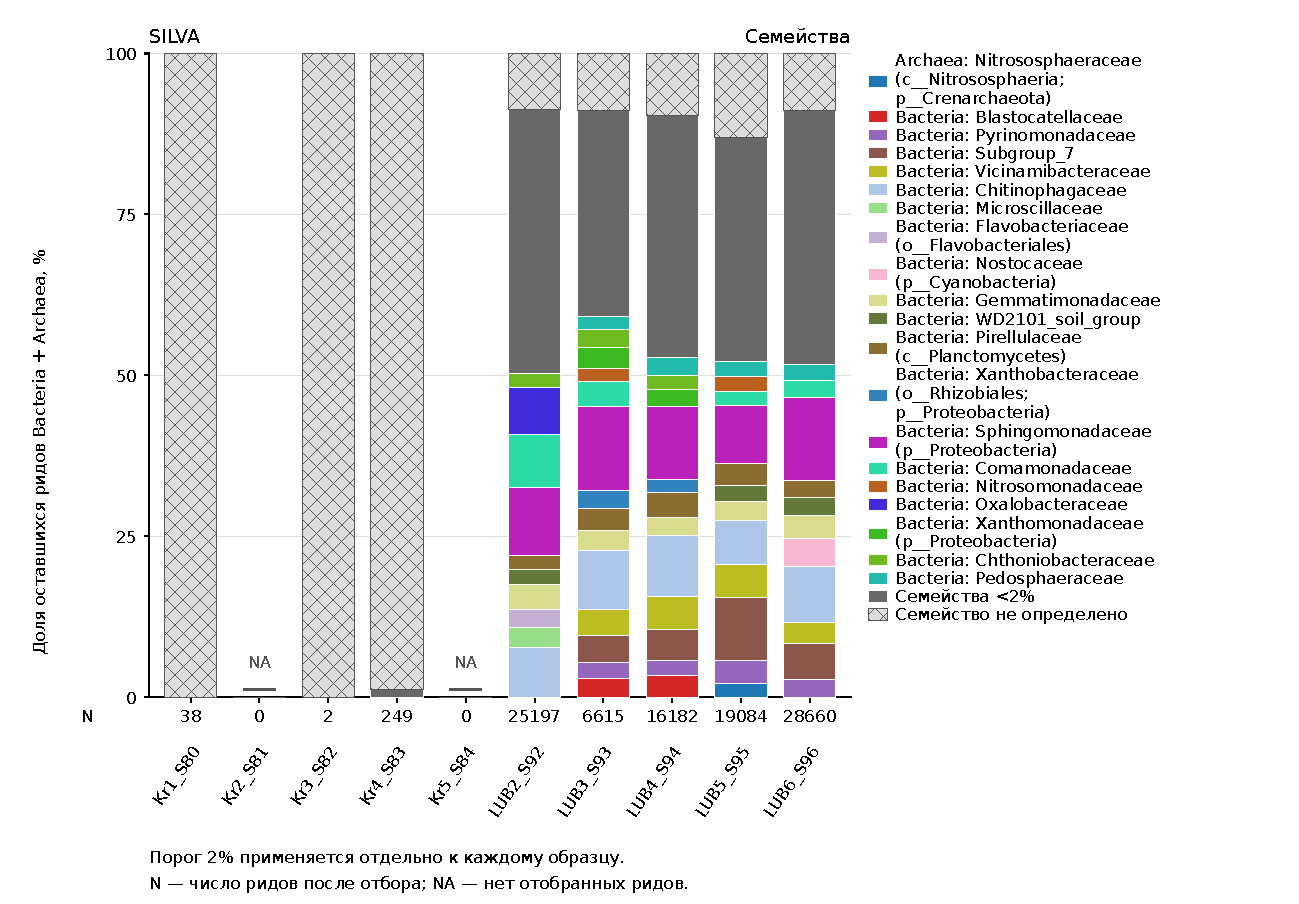
\includegraphics[width=\textwidth]{../../figures/taxonomy/family/prokaryotic_family_silva.pdf}
\caption{\porozhdeno{\Claim{F02}{Таксономические профили на уровне семейств по назначениям модели SILVA. Почвы после модельного отбора Bacteria + Archaea и исключения явно помеченных органелл; знаменатель каждого столбца --- его $N$. \texttt{UNCLASSIFIED} остаётся в знаменателе, точное \texttt{f\_\_uncultured} отнесено к нему; $N=0$ даёт NA. Семейства ниже \SelectedDisplayThresholdPct{}\% данного образца объединены без удаления ридов. Контроль не изображён.}}}
\label{fig:silva}
\end{figure}
\clearpage
\begin{figure}[!ht]
\centering
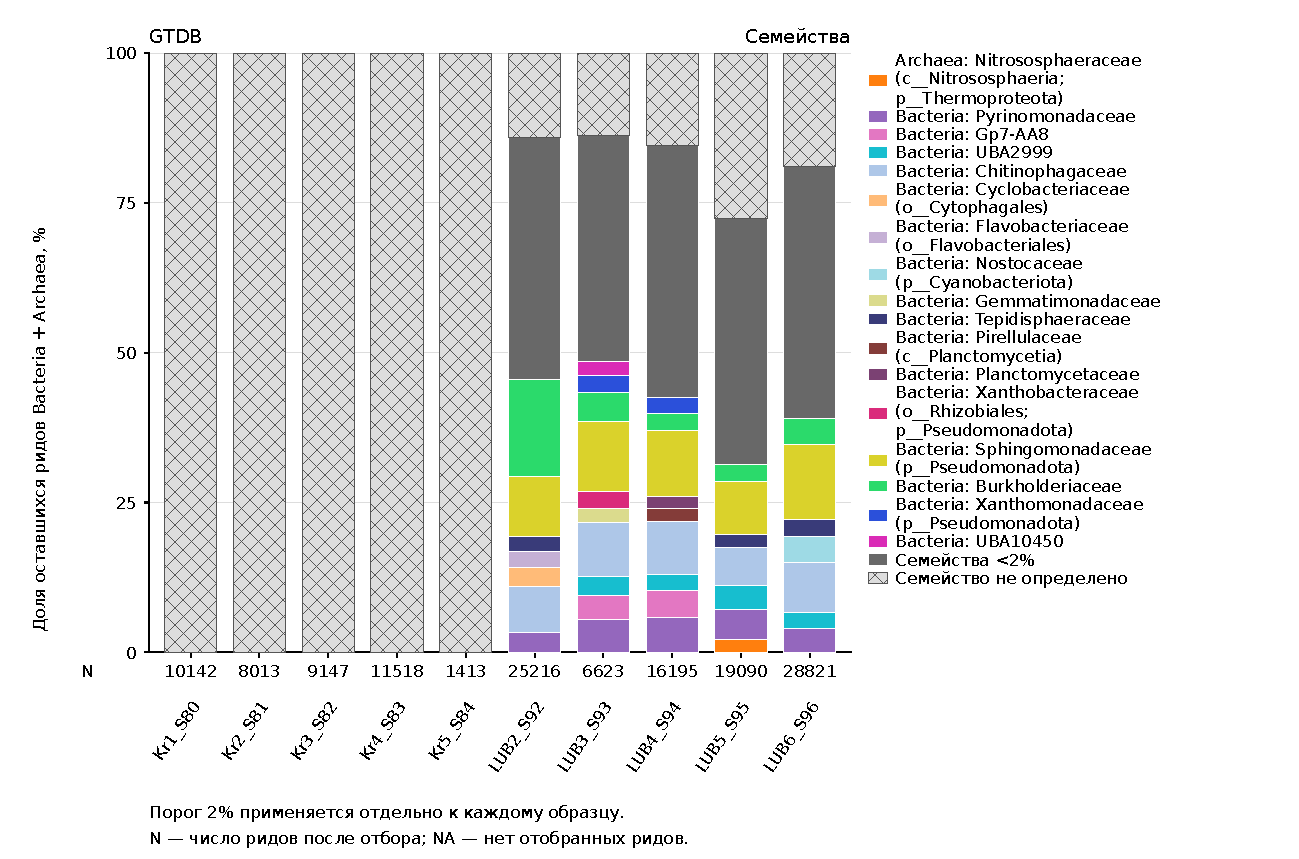
\includegraphics[width=\textwidth]{../../figures/taxonomy/family/prokaryotic_family_gtdb.pdf}
\caption{\porozhdeno{\Claim{F03}{Таксономические профили на уровне семейств по назначениям модели GTDB. Почвы после модельного отбора Bacteria + Archaea и исключения явно помеченных органелл; знаменатель --- собственный $N$ модели. \texttt{UNCLASSIFIED} включает неопределённые семейства и точное \texttt{f\_\_uncultured}; при $N=0$ доля была бы NA. Назначенные семейства ниже \SelectedDisplayThresholdPct{}\% сгруппированы без удаления ридов. Контроль исключён из рисунка.}}}
\label{fig:gtdb}
\end{figure}
\clearpage
\begin{figure}[!ht]
\centering
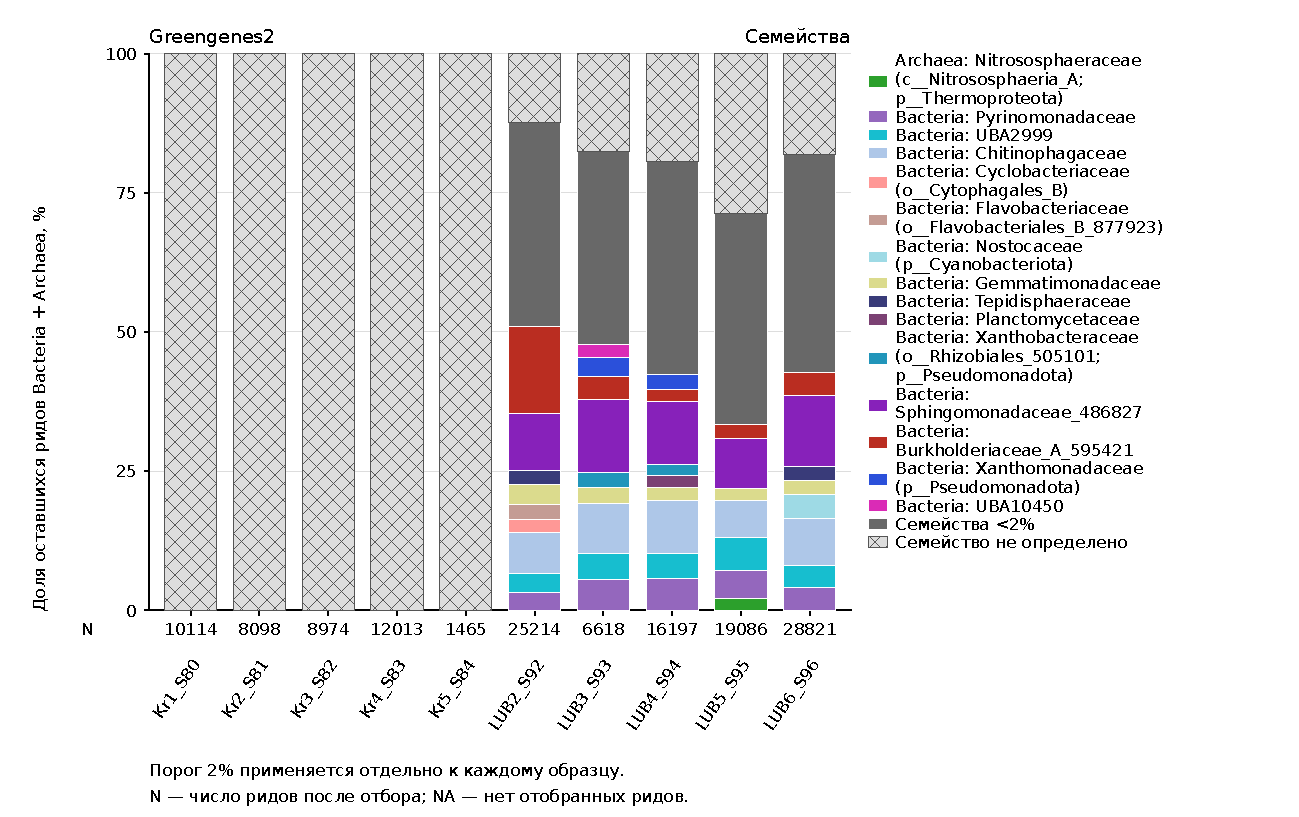
\includegraphics[width=\textwidth]{../../figures/taxonomy/family/prokaryotic_family_gg2.pdf}
\caption{\porozhdeno{\Claim{F04}{Таксономические профили на уровне семейств по назначениям модели Greengenes2. Почвы после модельного отбора Bacteria + Archaea и исключения явно помеченных органелл; знаменатель --- собственный $N$ модели с сохранённым \texttt{UNCLASSIFIED}, включая точное \texttt{f\_\_uncultured}. Пустой отбор означал бы NA. Назначенные семейства ниже \SelectedDisplayThresholdPct{}\% объединены серым, их риды остаются в $N$. Контроль не изображён.}}}
\label{fig:ggtwo}
\end{figure}

\end{document}
